\subsection{Lab17: BPSK}

%*********************
\begin{frame}{}

\pgfdeclareimage[width=\paperwidth,height=\paperheight]{bg}{imagenes/fondo_lab}
\setbeamertemplate{background}{\pgfuseimage{bg}}

\bfseries{\textrm{\LARGE Lab17\\ \Large BPSK}}
\raggedright
\end{frame}
%*************
%----------------------------------------
\begin{frame}

\pgfdeclareimage[width=\paperwidth,height=\paperheight]{bg}{imagenes/fondo3}
\setbeamertemplate{background}{\pgfuseimage{bg}}

\frametitle{\underline{\textbf{Modulación BPSK}}}

Para obtener una señal modulada se utiliza un modulador balanceado (Modulador de producto) que funciona como un conmutador, ya que a medida que la señal de información muestre un “1” o un “0” la portadora conmuta en dos fases diferentes. En un modulador BPSK se asigna +1 V al 1 lógico y -1 V al 0 lógico, la portadora de entrada, $\sin\omega_{c}t$se multiplica por +1 o por -1. En consecuencia, la señal de salida puede ser +1 $\sin\omega_{c}t$ o 1 $\sin\omega_{c}t$; el primer producto representa una señal que está en fase con el oscilador de referencia, y el último producto, una señal que está desfasada 180 grados [11]\\
La ecuación de salida de un modulador BPSK es proporcional a:\\

$$y(t)=[\sin(2 \pi f_{a}t)]X[\sin(2 \pi f_{c}t)]$$\\

\begin{enumerate}			
	\item{$f_{a}$: frecuencia fundamental máxima de la entrada binaria (señal moduladora) en hertz.}\\
	\item{$f_{c}$: frecuencia de portadora de referencia en hertz.}\\
\end{enumerate}
\end{frame}
%-----------------------------------------
\begin{frame}{Modulador BPSK en GRC}
\begin{figure}[H]
\vspace{-3mm}
\centering
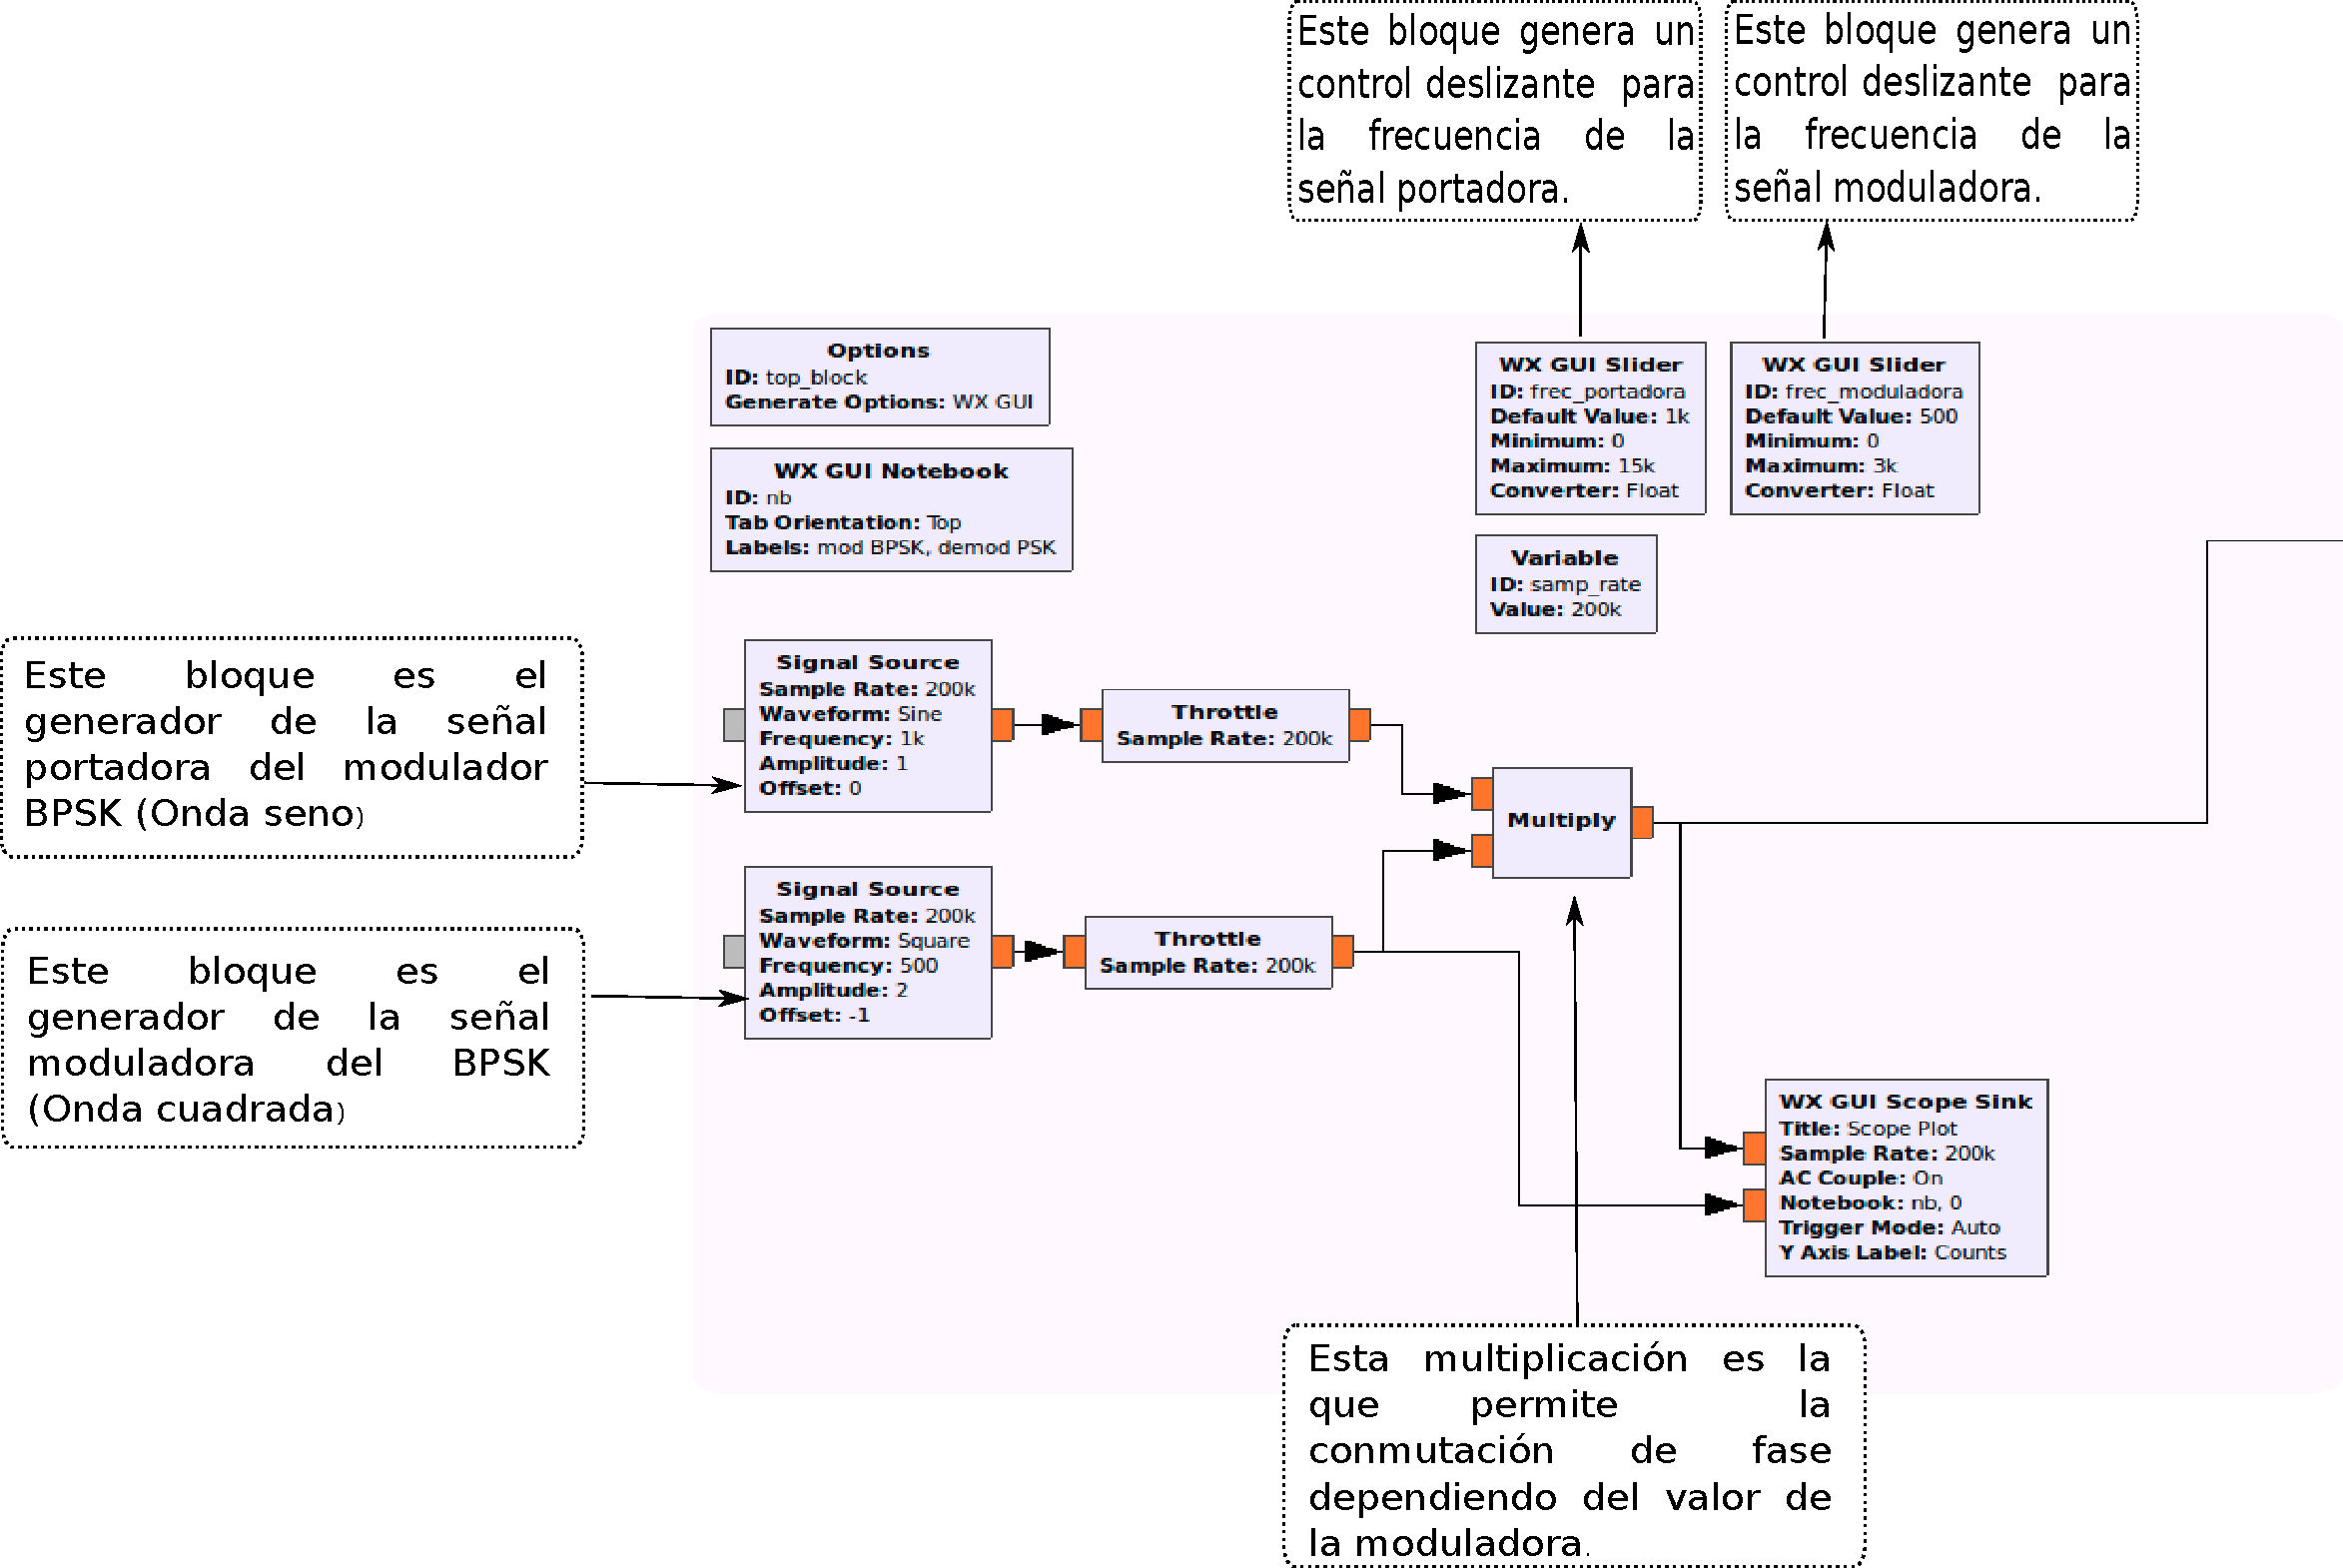
\includegraphics[width=0.9\textwidth]{Modulaciones_digitales/lab17/pdf/PSK_2.pdf}
\end{figure}
\end{frame}
%----------------------------------------
\begin{frame}{Modulación BPSK}
\begin{figure}[H]
\vspace{-3mm}
\centering
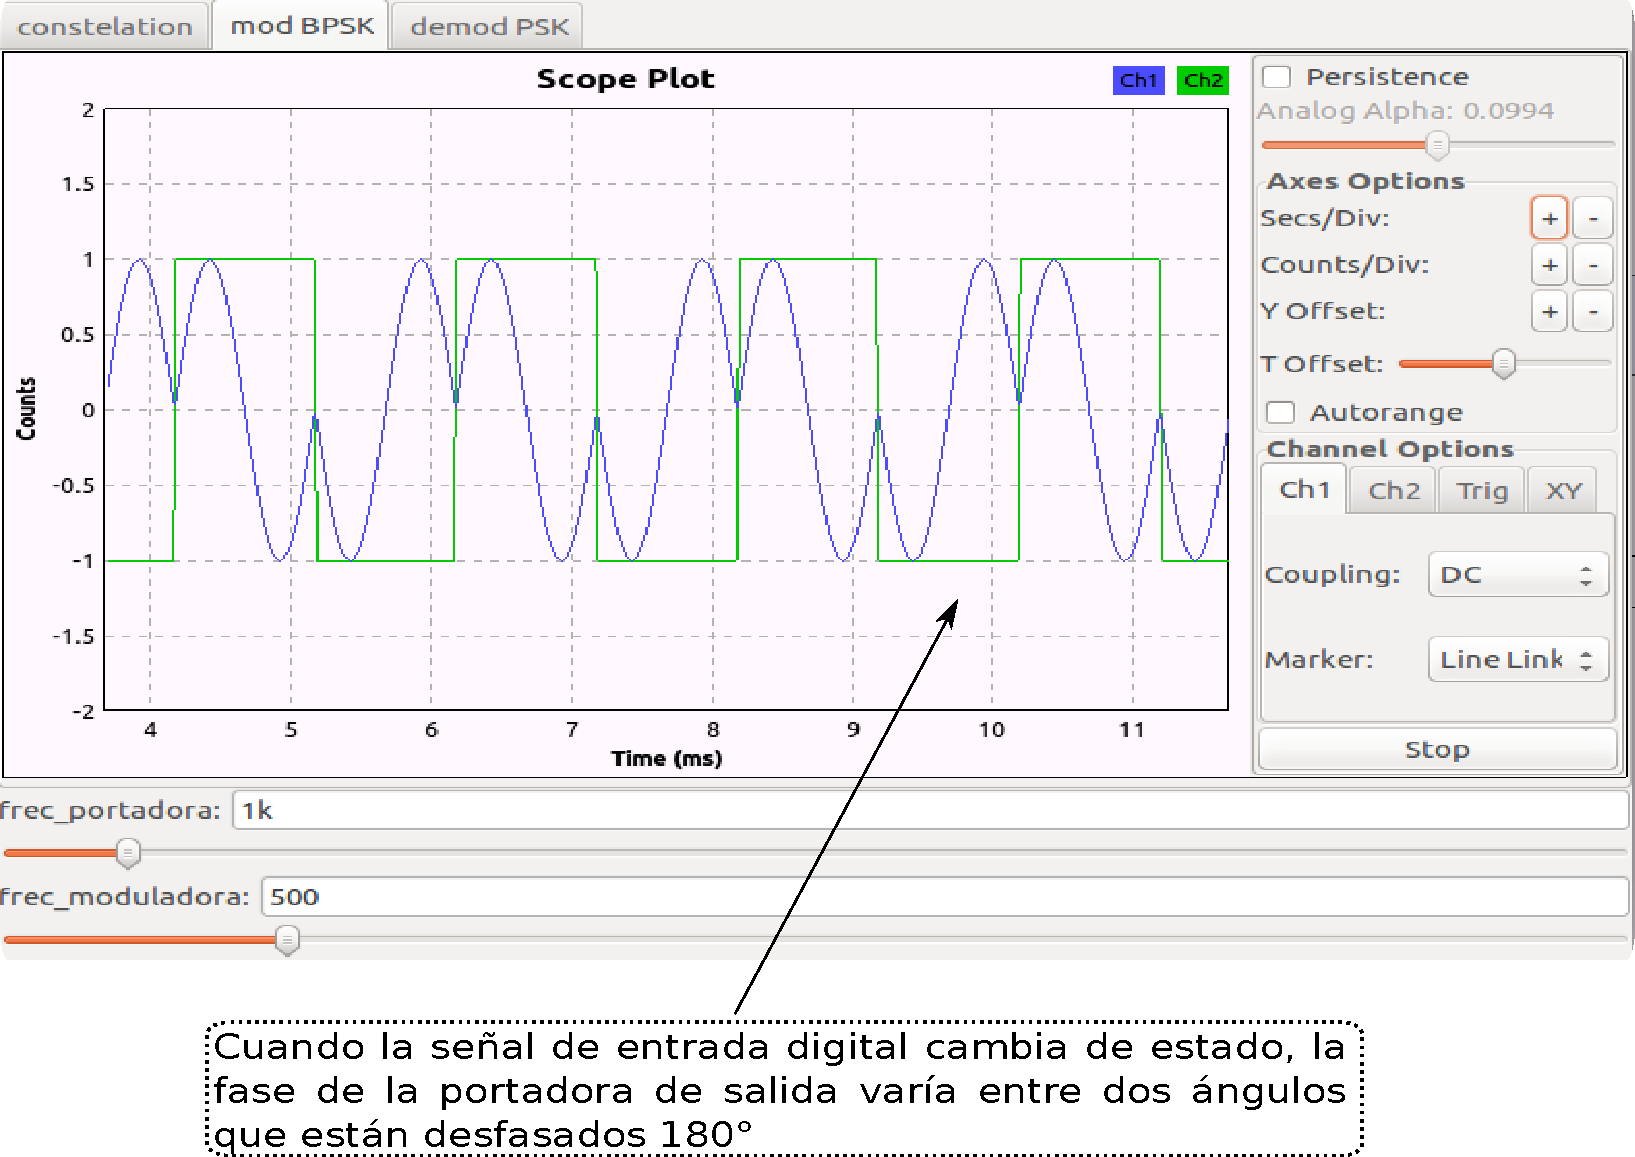
\includegraphics[width=0.9\textwidth]{Modulaciones_digitales/lab17/pdf/PSK_3.pdf}
\end{figure}
\end{frame}
%----------------------------------------
\begin{frame}

\pgfdeclareimage[width=\paperwidth,height=\paperheight]{bg}{imagenes/fondo3}
\setbeamertemplate{background}{\pgfuseimage{bg}}

\frametitle{\underline{\textbf{Demodulación BPSK}}}

El circuito de recuperación coherente de portadora detecta y regenera una señal de portadora que es coherente, tanto en fase como en frecuencia, con la portadora original de transmisión. El modulador balanceado es un detector de producto; la salida es el producto de las dos entradas (la señal BPSK y la portadora recuperada).El filtro pasabajas (LPF) separa los datos binarios recuperados de la señal demodulada.[11]

\end{frame}
%-----------------------------------------
\begin{frame}{Demodulador BPSK en GRC}
\begin{figure}[H]
\vspace{-3mm}
\centering
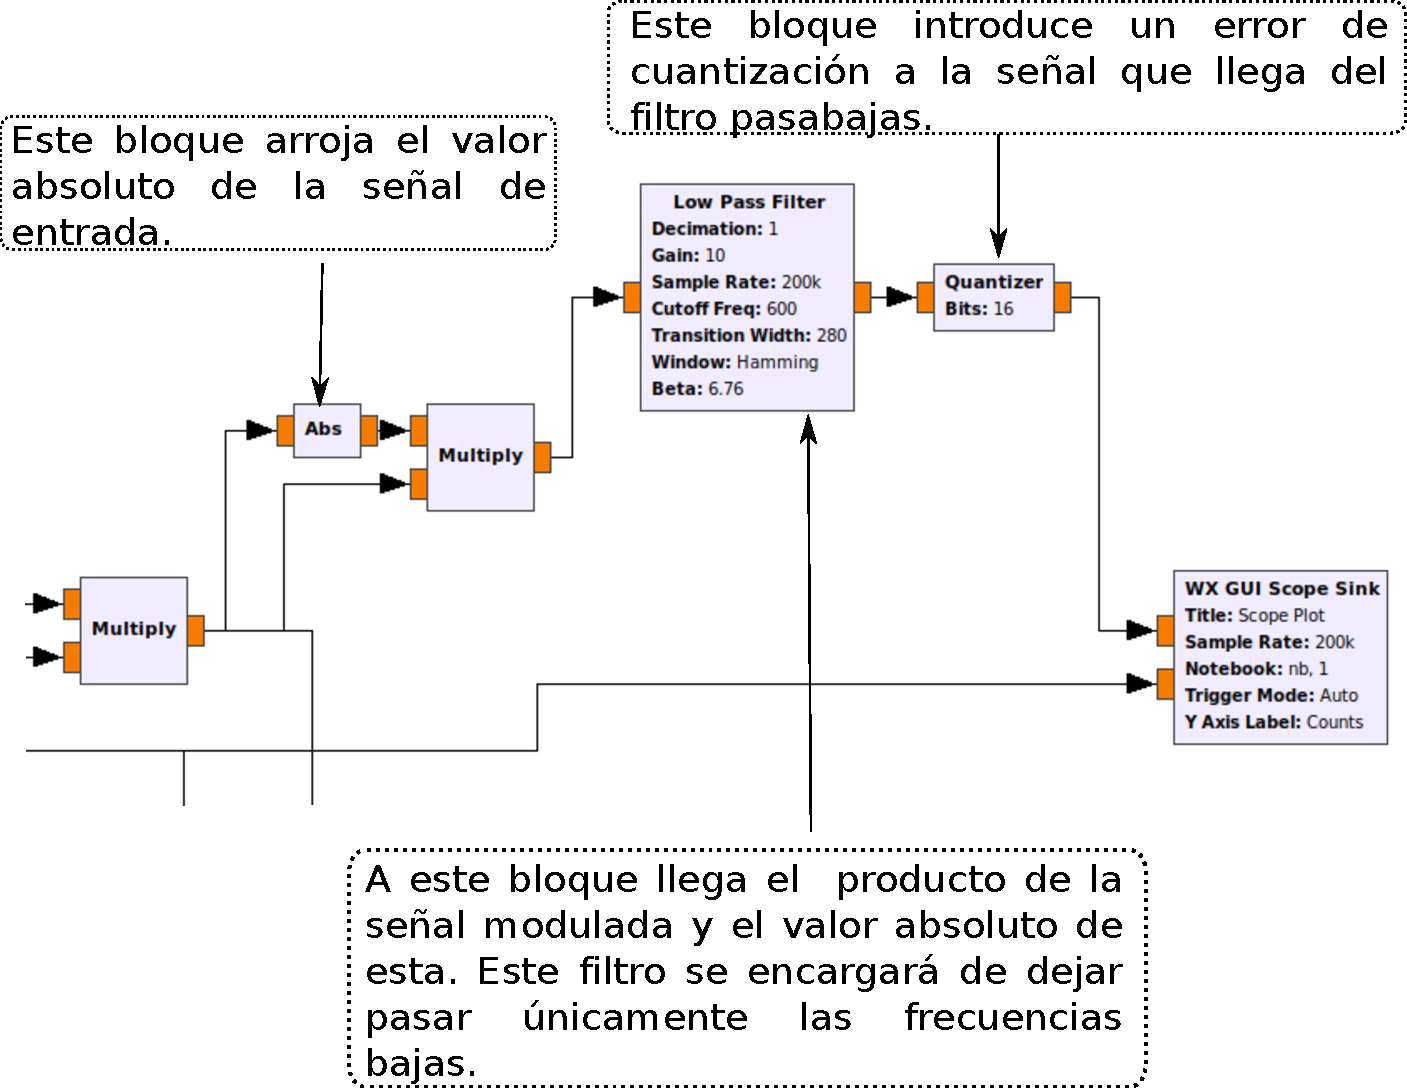
\includegraphics[width=0.8\textwidth]{Modulaciones_digitales/lab17/pdf/PSK_4.pdf}
\end{figure}
\end{frame}
%----------------------
\begin{frame}{Demodulación BPSK}
\begin{figure}[H]
\vspace{-3mm}
\centering
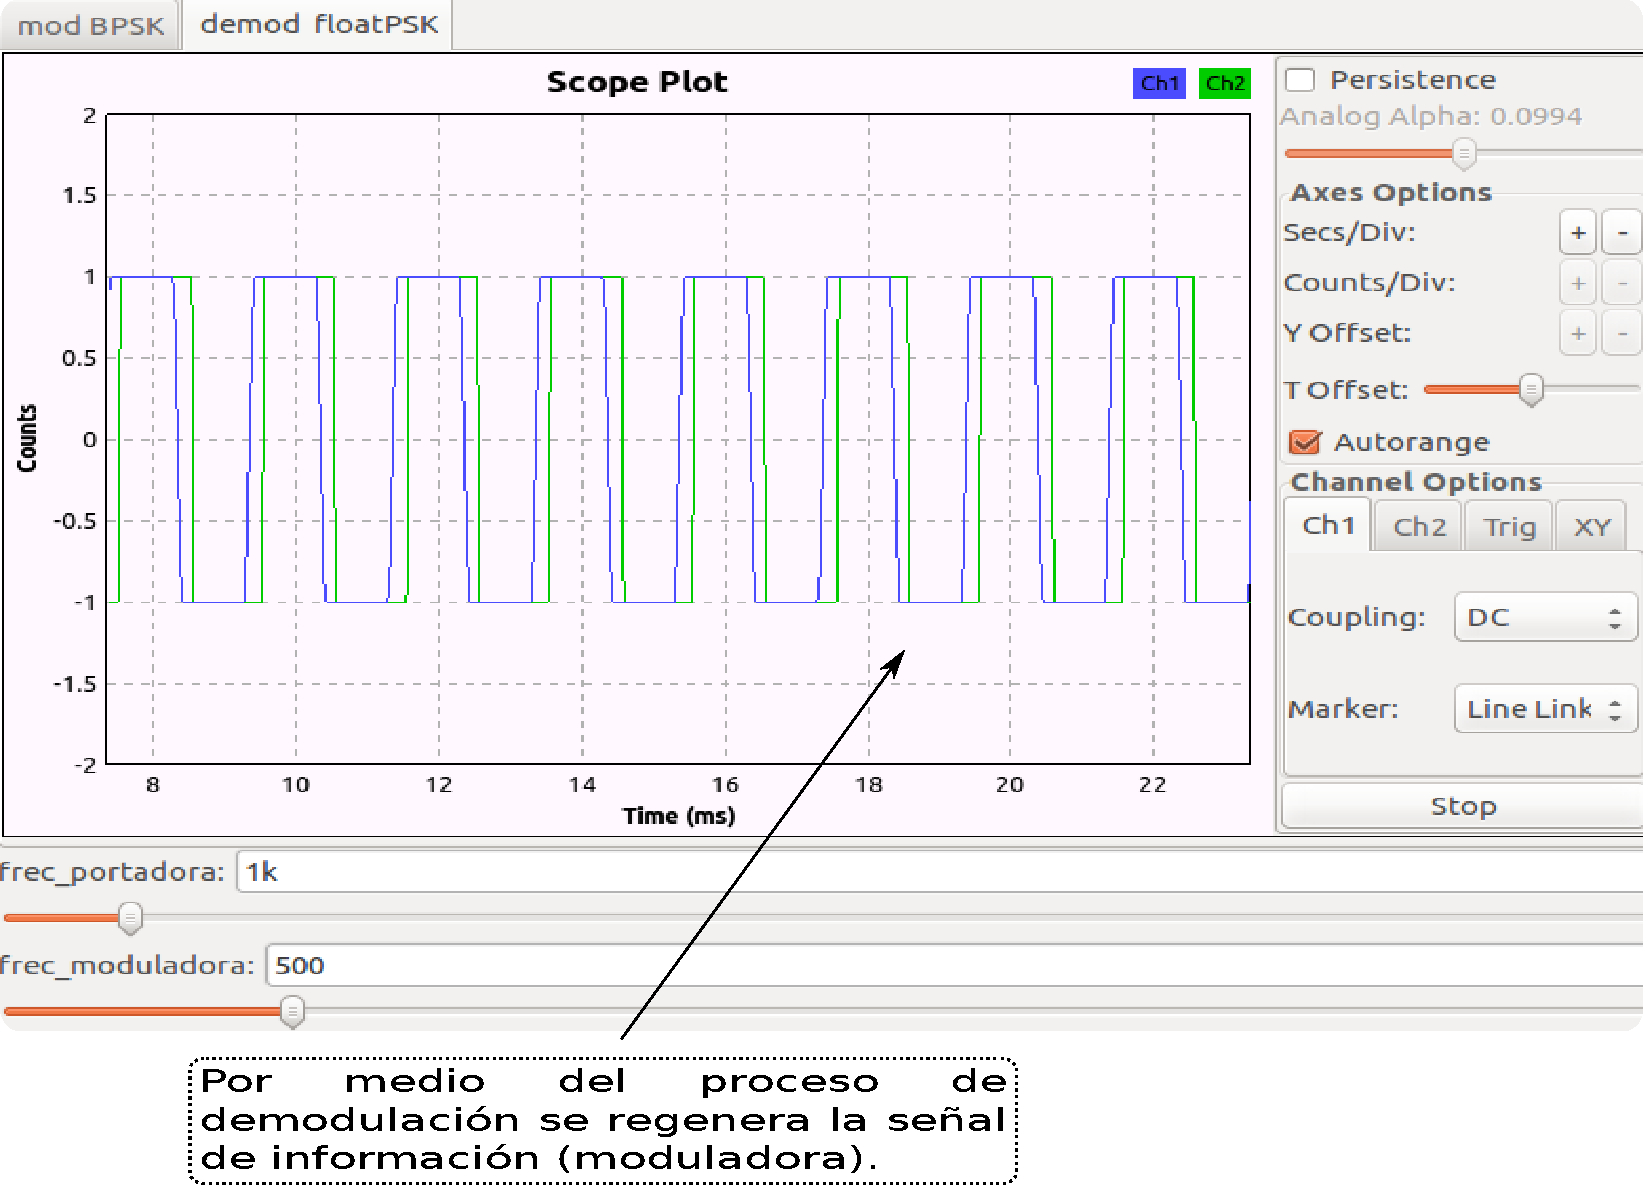
\includegraphics[width=0.9\textwidth]{Modulaciones_digitales/lab17/pdf/PSK_5.pdf}
\end{figure}
\end{frame}